\chapter{Logique booléenne}


\section{Introduction}

\begin{wrapfigure}[7]{r}{3.5cm}
  \vspace{-20mm}
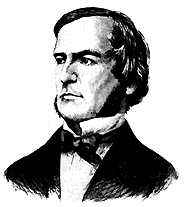
\includegraphics[width=4cm]{./figures/george_boole.jpg}
\end{wrapfigure}
Nous nous intéressons ici à une algèbre sur les propositions logiques : nous serons à même d'effectuer des calculs sur la logique à 2 valeurs : vrai ou faux.
C'est George Boole qui l'introduisit au milieu du \siecle{19}. Connu pour ses travaux sur les équations différentielles, il l'est encore plus lorsqu'il fait paraître
un traité qui fit date, intitulé {\it "An Investigation Into the Laws of Though"}, au titre très annonciateur. Son intention sous-jacente était de traduire des
idées et concepts en équations, puis d'effectuer des calculs sur la véracité de ces idées : là aussi, on peut rester admiratif devant tant d'intuition !
Pourtant, il semble que ses travaux sont longtemps restés cantonnés à des jeux de salons mondains.
A titre d'exemple, voici une énigme qui peut être résolue grace à l'algèbre de Boole :
on dispose de 3 boîtes A,B et C et de 3 jetons de couleur respective bleu, blanc et rouge. Chaque boîte possède un jeton. Sachant qu'une seule
proposition est vraie, déterminer le contenu de chaque boîte.

\begin{enumerate}
  \item la boîte A contient le jeton rouge.
  \item la boîte B ne contient pas le jeton rouge
  \item la boîte C ne contient pas le jeton bleu.
\end{enumerate}

Cette logique s'appelle également la {\it logique des propositions}. On pourra mettre en relation (on dit aussi "connecter") ces propositions grâce à l'algèbre de Boole.
C'est seulement au  \siecle{20} que Claude Shannon redécouvrit le pouvoir de modélisation de l'algèbre de Boole et son applicabilité
directe au domaine de l'Electronique.

\section{Définitions}


Soit $\mathbb{B}=\{0,1\}$ l'espace de Boole. Une variable booléenne simple est définie sur $\mathbb{B}.$
Il est également possible de travailler sur plusieurs variables : une variable booléenne {\bf générale} est un n-uplet $X=(x_1,x_2,\dots,x_n) \in \mathbb{B}$ et peut prendre $2^n$ valeurs. L
a valeur de $X$ est appelée un point. Un litéral est une variable booléenne simple ou son complément. Par exemple, $a$ et $\overline{a}$ sont deux littéraux distincts correspondant à la même
 variable.\\

Les opérations de l'algèbre de Boole sont les suivantes :
\begin{itemize}
\item La {\bf Conjonction} (ou produit logique) de deux variables (bits) : on parlera plus volontiers du {\bf ET} logique, dénoté par un signe croix ($\times$).
\item La {\bf Disjonction} (ou somme logique) de deux variables (bits) : on parlera plus volontiers du {\bf OU} logique, dénoté par un signe plus ($+$).
\item La {\bf Négation} (ou complémentation ou inversion) d'un seul bit : on parlera plus volontiers du {\bf NON}, dénoté par une barre au dessus de la variable ($\bar a$).
\end{itemize}

Ces opérations peuvent être représentées par des {\bf tables de vérité}, qui énumèrent explicitement les correspondances entre les entrées et les sorties :

\begin{center}
\begin{tabular}{|c c|c|}
  \hline
  $a$ & $b$  & $a \times b$ \\
  \hline
  0 & 0 & 0 \\
  0 & 1 & 0 \\
  1 & 0 & 0 \\
  1 & 1 & 1 \\
  \hline
\end{tabular}
\quad
\begin{tabular}{|c c|c|}
  \hline
  $a$ & $b$  & $a + b$ \\
  \hline
  0 & 0 & 0 \\
  0 & 1 & 1 \\
  1 & 0 & 1 \\
  1 & 1 & 1 \\
  \hline
\end{tabular}
\quad
\begin{tabular}{|c|c|}
  \hline
  $a$ & $\bar{x}$ \\
  \hline
  0 & 1 \\
  1 & 0 \\
  \hline
\end{tabular}
\end{center}

$x \times y$ vaut $1$ si $x$ vaut 1 {\bf et}  $x$ vaut 1, $0$ sinon.

$x + y$ vaut $1$ si $x$ vaut 1 {\bf ou}  $x$ vaut 1, $0$ sinon.

$\bar{x}$ vaut $1$ si $x$ vaut 0, $0$ sinon.

Il est à noter que le OU logique n'a pas la même signification ici et dans le langage de la rue : lorsqu'on utilise le OU dans la vie de tous les jours, il s'agit d'une exclusion (c'est l'un
e ou l'autre des variables qui est sensée être vraie). On parlera alors de OU {\it exclusif}, alors que le OU ($+$) est un OU {\it inclusif}. Retenez toutefois que le OU {\it exclusif} est é
galement utilisable et utilisé en électronique. Son symbole est généralement le $\oplus$.

\subsection{Axiomes de l'Algèbre de Boole}
Soit {\it x,y,z} des variables booléennes. Les axiomes de l'Algèbre de Boole sont les suivants :

\begin{enumerate}
%% \item Alors $x = 0$ ou $x = 1$ . Si $x=0$, alors $\bar{x} = 1$ , et vice versa.
%% \item $0 \times 0 = 0$
%% \item $0 \times 1 = 1 \times 0 = 0$
%% \item $1 \times 1 = 1$
%% \item $0 + 0 = 0$
%% \item $0 + 1 = 1 + 0 = 1$
%% \item $1 + 1 = 1$
\item  {\bf $+$ est associatif} :  $x+(y+z)=(x+y)+z$
\item  {\bf $\times$ est associatif} :  $x\times(y\times z)=(x\times y)\times z$
\item  {\bf $+$ est commutatif} :  $x+y=y+x$
\item  {\bf $\times$ est commutatif} :  $x\times y=y\times x$
\item  {\bf existence d'un élément neutre pour $+$} :  $\exists 0 / x+ 0 = x$
\item  {\bf existence d'un élément neutre pour $\times $} :  $\exists 1 / x \times 1 = x$
\item  {\bf $\times$ est distributif sur $+$} : $x.(y+z)=x.y+x.z$
\item  {\bf $+$ est distributif sur $\times$} : $x+(y.z)=(x+y).(x+z)$. Ce résultat est plus surprenant !
\item  {\bf existence du complément}
\end{enumerate}

\subsection{Principaux théorèmes de l'Algèbre de Boole}

\begin{enumerate}
\item {\bf $+$ est idempotent} : $x+x=x$
\item {\bf $\times$ est idempotent} : $x \times x=x$
\item {\bf $1$ est absorbant pour $+$} : $x+1=1$
\item {\bf $0$ est absorbant pour $\times$} : $x\times 0=0$
\item {\bf unicité du complément}
\item {\bf complément du complément} : $\overline{ ( \overline{x} ) }=x$
\item $x+x.y = x$
\item $x \times (x + y) = x$
\item $x + \bar{x} \times y = x +y$
\end{enumerate}

\subsection{Théorèmes de De Morgan}

Parmi les théorèmes de l'algèbre de Boole, les théorèmes de de Morgan sont particulièrement intéressants et utiles pour la suite.
Observons le tableau suivant, qui expose le calcul de deux fonctions $f_1(a,b)=\overline{a+b}$ et $f_2(a,b)=\overline{a}.\overline{b}$.

\begin{center}
   \begin{tabular}{|c|c|c|c|c|c|c| }
     \hline
     a & b & $a+b$ & $f_1=\overline{a+b}$ & $\overline{a}$ & $\overline{b}$ & $f_2=\overline{a}.\overline{b}$ \\ \hline \hline
     0 & 0 &     0 &                   1  &              1 &              1 &                              1  \\ \hline
     0 & 1 &     1 &                   0  &              1 &              0 &                              0  \\ \hline
     1 & 0 &     1 &                   0  &              0 &              1 &                              0  \\ \hline
     1 & 1 &     1 &                   0  &              0 &              0 &                              0  \\ \hline
   \end{tabular}
 \end{center}

Ce calcul démontre que les deux fonctions sont en fait égales :
$$\boxed{\overline{a+b}=\overline{a}.\overline{b}}$$
On peut également démontrer que :
$$\boxed{\overline{a.b}=\overline{a}+\overline{b}}$$

Ce résultat peut bien entendu se généraliser pour plus de 2 variables. La manière de retenir se résultat consiste à s'apercevoir que
"la descente de la barre sur les opérandes" s'accompagne du changement de l'opération "+" en "*" (et vice versa)

\section{Représentation des fonctions booléennes}

\subsection{Monôme}
Un monôme $m$ est un produit de $p$ variables simples distinctes sous formes normales ($x$) ou complémentées ($\overline{x}$). Un monôme canonique est un monôme de degré $n$ dans $\mathbb{B}
^n$.

\subsection{Fonctions booléennes}
Une fonction booléenne est une fonction de $\mathbb{B}^n$ vers $\mathbb{B}^m$.

\begin{itemize}
\item $n=1,m=1$ : la fonction est dite fonction simple d'une variable simple.
\item $n>1,m=1$ : la fonction est dite fonction simple d'une variable générale.
\item $n>1,m>1$ : la fonction est dite fonction générale d'une variable générale.
\item $n=1,m>1$ : la fonction est dite fonction générale d'une variable simple.
\end{itemize}

{\bf Exemple} : la fonction $F(a,b)=a+b$ est une fonction booléenne simple d'une variable générale $(a,b)$

\subsection{Fonction booléenne incomplète ou $\phi$-booléenne}

Si $F$ n'est pas définie en $X\in \mathbb{B}^n$, on a l'habitude de poser $F(X)=\phi$, où $\phi$ représente à la fois $0$ et $1$ superposés. $\phi$ représente la valeur indéfinie (en anglais
 ``don't care''), qui signifie que la fonction peut prendre indistinctement la valeur $0$ ou $1$ en ce point. On dit que $F$ couvre un point $X$ si $F(X)=1$.

\subsection{Minterm et maxterms}
Nous avons établi qu'une variable booléenne peut apparaître sous sa forme normale ou complémentée.
Par ailleurs, le produit de deux variables $A$ et $B$ conduit à $2^2=4$ combinaisons possibles : $A.B,\overline{A}.B,A.\overline{B}$ et $\overline{A}.\overline{B}$. Ces $4$ s'illustrent sur
un diagramme de Venn. Ces $4$ produits sont des {\it minterms} ou {\it produits standards}. En d'autres mots, un minterm est un produit composé de deux variables (ou plus) ou de leur complém
ents.

\subsection{Décomposition de Shannon et Arbres de décision binaires}
La décomposition de Shannon ne sera pas utilisée dans ce cours, mais mérite toutefois d'être évoquée. En effet, elle est à la base des représentations manipulables par les ordinateurs : il f
aut se projeter dans des systèmes numériques composés de millions d'équations logiques, pour lesquels il est important de manipuler efficacement ces notions ! Cette décomposition s'écrit de
la manière suivante :

$$F(x_1,x_2,\dots,x_n)=x_1.F(1,x_2,\dots,x_n) + \overline{x_1}.F(0,x_2,\dots,x_n)$$

%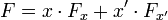
\includegraphics[scale=0.5]{../figures/shannon_0.png}
%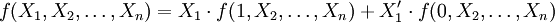
\includegraphics[scale=0.5]{../figures/shannon.png}

Son intérêt est qu'il est possible de l'appliquer récursivement. Cette décomposition s'illustre de la manière suivante , appelée diagrammes (ou arbres) de décisions binaires (BDD : binary de
cision diagrams) :

%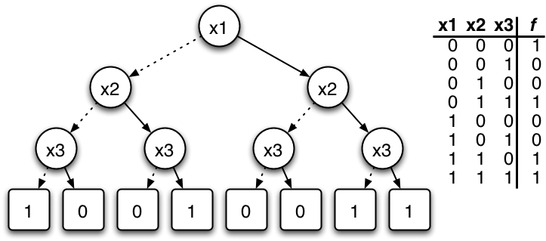
\includegraphics[scale=0.3]{../figures/bdd.jpg}

Cette décomposition a permi l'essor d'outils de preuves formelles sur les circuits --mais pas seulement-- : les ``solvers'' de satisfiabilité par exemple permettent de trouver s'il existe un
e variable totale qui rende une formule booléenne vraie (problème SAT). C'est un problème très difficile \footnote{SAT est le premier problème connu dit NP-complet...} !

En réalité, le terme de BDD est généralement associé à ROBDD : Reduced Ordered Binary Decision Diagram. L'intérêt des ROBDD est qu'il présente une forme canonique (unique) pour une fonction
donnée et quel que soit l'ordre d'évaluation des variables. Cette propriété le rend très utilse dans la recheche d'équivalence entre 2 circuits : implémentent-ils intrinsèquement la même for
mule, bien qu'ils se présentent sous une forme électronique différente ?

%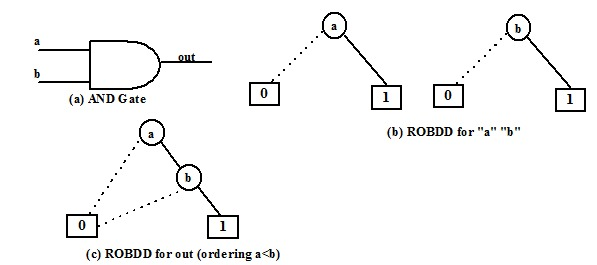
\includegraphics[scale=0.3]{../figures/robdd_and.jpg}
%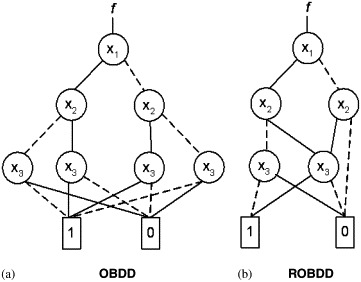
\includegraphics[scale=0.3]{../figures/obdd.jpg}
%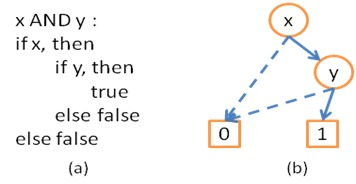
\includegraphics[scale=0.3]{../figures/bdd-prog.jpg}

\section{Simplification des fonctions booléennes}

\subsection{Par calcul algébrique}

La simplification d'expressions booléennes est un exercice difficile --y compris pour les ordinateurs qui les effectuent--, mais qui est nécessaire pour
optimiser le matériel. L'exemple suivant montre un exemple minuscule. Les deux signaux de sortie sont totalement identiques du point de vue logique : en fait
, on n'avait besoin d'aucune porte logique !

\begin{center}
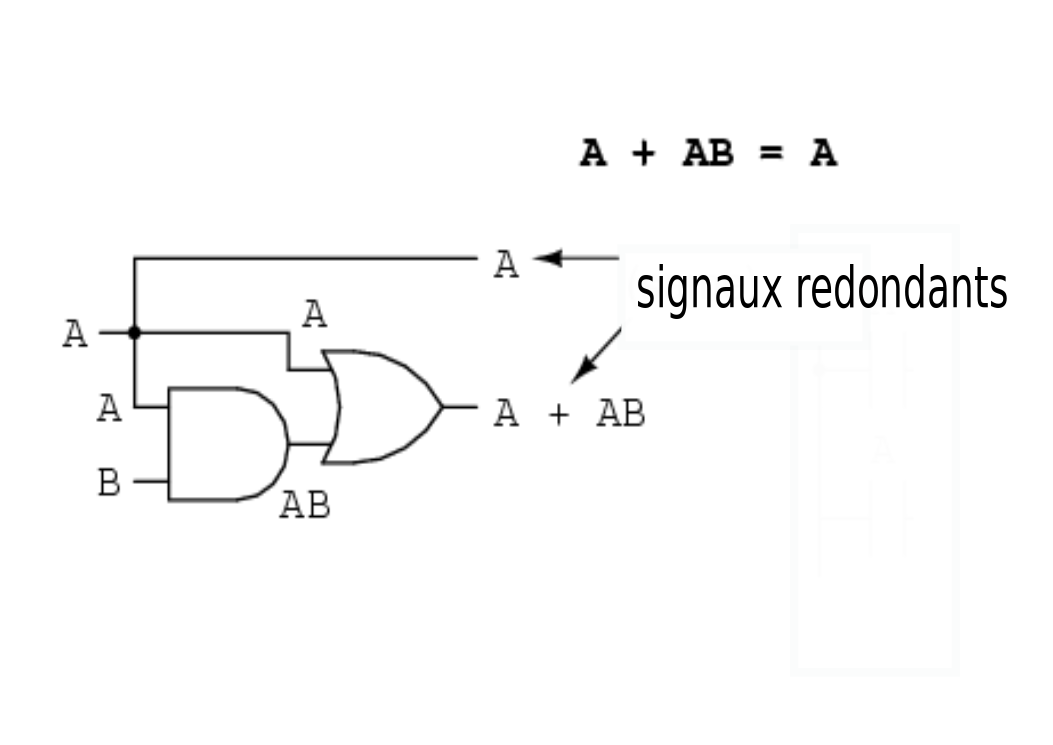
\includegraphics[scale=0.2]{./figures/redondance.png}
\end{center}

Cet exemple suggère également comment simplifier le circuit, par application des règles de composition algébrique vues précédemment. Voici le cheminement que l'on peut utiliser :
\begin{enumerate}
\item $A+A\times B$. Factorisons par $A$
\item $A(1+B)$. Appliquons l'identité $1+B=1$
\item $A\times 1$. Il s'en suit :
\item $A$
\end{enumerate}

Toutefois, la bonne application successive de ces règles est difficile pour des formules complexes. Cette application dépend de votre capacité à ``sentir'' la simplification...Il existe heur
eusement une autre méthode, plus mécanique.

\subsection{Par tableau de Karnaugh}
Les tableaux de Karnaugh permettent d'appliquer de manière mécanique des simplifications qui marchent à coup sûr. Ces tableaux sont en fait un ensemble de cases.
En général, une expression booléenne à $n$ variables peut être représentées par un tableau de Karnaugh à $2n$ cases, où chaque case représente une ligne d'une
table de vérité équivalente. Dans la méthode des tableaux de Karnaugh, il est nécessaire de disposer les entrées du tableaux d'une manière particulière : sans
cette disposition spéciale, la méthode ne peut s'appliquer. Cette manière particulière consiste à s'arranger afin que des cases contigues ne diffèrent que
d'une seule variable. On retrouve ici le code de Gray. Lorsque les entrées sont correctement énumérées, on peut disposer les monômes de la fonction à simplifier
dans ce tableau. Il est recommandé d'écrire au préalable la fonction logique sous la forme de sa table de vérité : il ne faudra pas confondre cette table de vérité initiale
et le tableau de Karnaugh associé ! Placer les monomes dans le tableau consiste à détecter les '1' de la fonction, dans sa table de vérité, et disposer ces '1' dans le tableau
de Karnaugh. Dès lors de ces monômes sont correctement reportés dans le tableau, on cherche des regroupements de '1' : on cherche précisément les regroupements
de '1' qui présentent un nombre d'éléments qui soit une puissance de 2 : 2, 4, 8 , 16 etc...  Ces regroupements doivent être soigneusement entourés. Du fait de l'adjacence des entrées du tableau, ces regroupements induisent
une simplification. Plus le nombre d'éléments regroupés est élevé, plus les simplifications seront importantes. Si aucun regroupement n'est possible, cela signifie qu'aucune simplification
ne peut s'appliquer.\\

Avant de nous lancer, prenons soin de remarquer que l'adjacence des cases fonctionne également sur les bords des tableaux : le haut et le bas sont adjacents ! Ainsi que la gauche et la droite ! Mieux encore,
les 4 angles sont également adjacents. Cela signifie qu'un ensemble de quatre '1' disposés aux quatre angles se prêtent à une simplifications booléenne.\\

Observons un premier cas : simplifions la fonction $f_1(a,b,c)=a.b.\overline{c}+a.b.c$. La simplifications algébrique est ici triviale, mais passons par un tableau de Karnaugh.
Les deux monômes, disposés dans le tableau, permettent un regroupement de 2 cases. La variable 'c' est ici simplifiable, {\it du fait de cette adjacence} (le retour à la méthode algébrique le confirme). La fonction
vaut donc au final $f_1(a,b,c)=a.b$.\\

\begin{center}
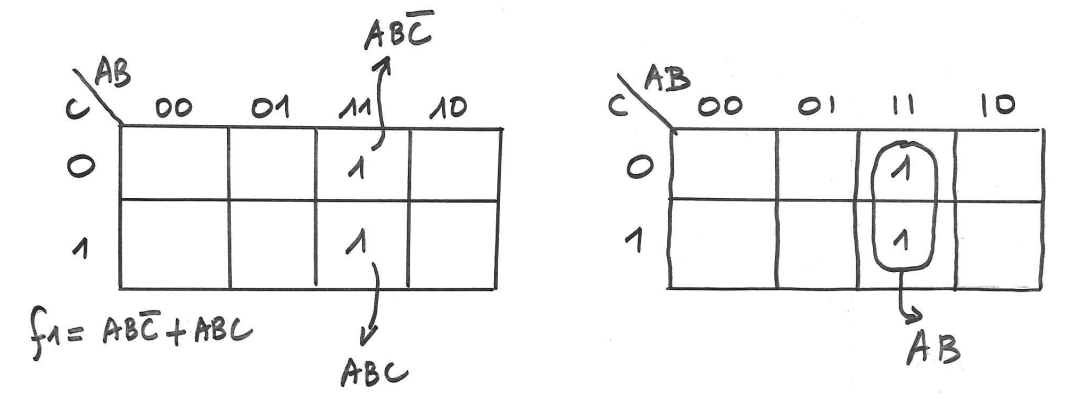
\includegraphics[scale=0.2]{./figures/karnaugh_00.png}
\end{center}

On peut s'autoriser désormais à utiliser cette méthode pour des simplifications moins triviales.
Ainsi, la fonction $f(a,b,c,d)=a.b+\overline{a}.b.\overline{c}.d+\overline{a}.b.c.d + a.\overline{b}.\overline{c}.\overline{d}$ vaut,
simplifiée $f(a,b,c,d)=a.b+b.d+a.\overline{c}.\overline{d}$
\begin{center}
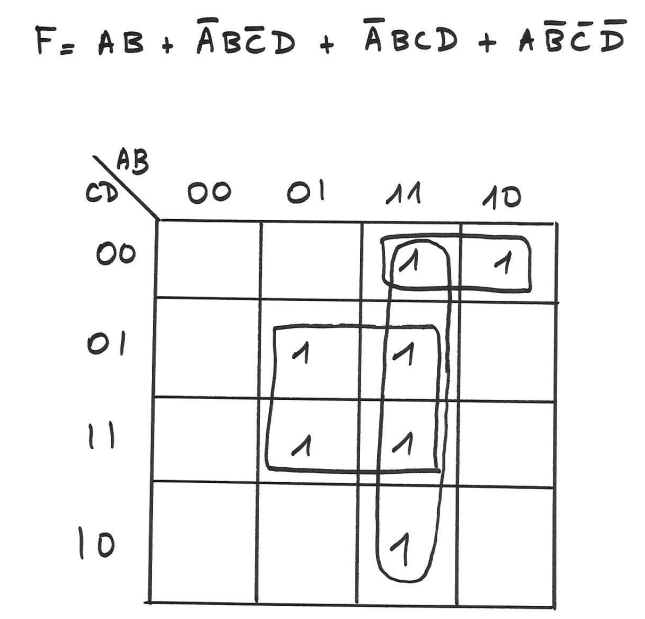
\includegraphics[scale=0.2]{./figures/karnaugh_01.png}
\end{center}


%% \subsection{Autres méthodes}
La bonne nouvelle est que ces simplifications ont été automatisées dans des logiciels.
Au cours de l'Histoire, plusieurs méthodes ont vu le jour : notamment l'algorithme de Quine Mac Cluskey, puis des méthodes symboliques, à base de BDD, encore plus puissantes.
Toutefois, les algorithmes soulèvent des problèmes de
complexité informatique insoupçonnés : il n'existe pas de méthodes qui puisse garantir le caractère optimal du résultat, pour tous les cas !

\section{Conclusion}
Ce chapitre nous a permis de nous familiariser avec l'algèbre de Boole. Il s'agit là de bases essentielles
à la mise en équation de problèmes d'électronique numérique. Ce socle solide va nous permettre d'aborder l'ensemble de la conception en Electronique
et Informatique (embarquée ou non) de manière sereine. Dans le chapitre suivant, nous allons directement chercher à représenter ces équations issues
de l'algèbre de Boole par de véritables circuits électroniques.
